\documentclass{beamer}

\usefonttheme{professionalfonts} % using non standard fonts for beamer
\usefonttheme{serif} % default family is serif

\usepackage{enumitem}
\setitemize{label=\usebeamerfont*{itemize item}%
  \usebeamercolor[fg]{itemize item}
  \usebeamertemplate{itemize item}}

\usepackage{hyperref}
%\usepackage{minted}
\usepackage{animate}
\usepackage{graphicx}
\def\Put(#1,#2)#3{\leavevmode\makebox(0,0){\put(#1,#2){#3}}}
\usepackage{colortbl}
\usepackage{tikz}
\usepackage{amssymb}
\usepackage{enumerate}
\usepackage{arydshln}
\usepackage{algorithm}
\usepackage{algpseudocode}
\usepackage{subcaption} %to have subfigures available

\usepackage[absolute,overlay]{textpos}

\colorlet{lightred}{red!25}
\colorlet{lightgreen}{green!25}
\beamertemplatenavigationsymbolsempty

\newcommand\blfootnote[1]{%
  \begingroup
  \renewcommand\thefootnote{}\footnote{#1}%
  \addtocounter{footnote}{-1}%
  \endgroup
}

\makeatletter

%% Textclass specific LaTeX commands.
\newcommand\makebeamertitle{\frame{\maketitle}}%
\AtBeginDocument{%
  \let\origtableofcontents=\tableofcontents
  \def\tableofcontents{\@ifnextchar[{\origtableofcontents}{\gobbletableofcontents}}
  \def\gobbletableofcontents#1{\origtableofcontents}
}
%% User specified LaTeX commands.
\usetheme{Malmoe}
\useoutertheme{infolines}
\addtobeamertemplate{headline}{}{\vskip2pt}
\setbeamercovered{transparent}

\title[PFlock report]{PFLOCK Report}
\author[AC]{Andres Calderon}
\institute[UCR]{University of California, Riverside}
\makeatother

%%%%%%%%%%%%%%%%%%%%%%%%%%%%%%%%%%%%%%
%% Main document
%%%%%%%%%%%%%%%%%%%%%%%%%%%%%%%%%%%%%%
\begin{document}
\makebeamertitle
\newif\iflattersubsect

\AtBeginSection[] {
    \begin{frame}<beamer>
    \frametitle{Outline} 
    \tableofcontents[currentsection]  
    \end{frame}
    \lattersubsectfalse
}

\AtBeginSubsection[] {
    \begin{frame}<beamer>
    \frametitle{Outline} 
    \tableofcontents[currentsubsection]  
    \end{frame}
}

\begin{frame}{Benchmark DBScan implementations}
    \centering
    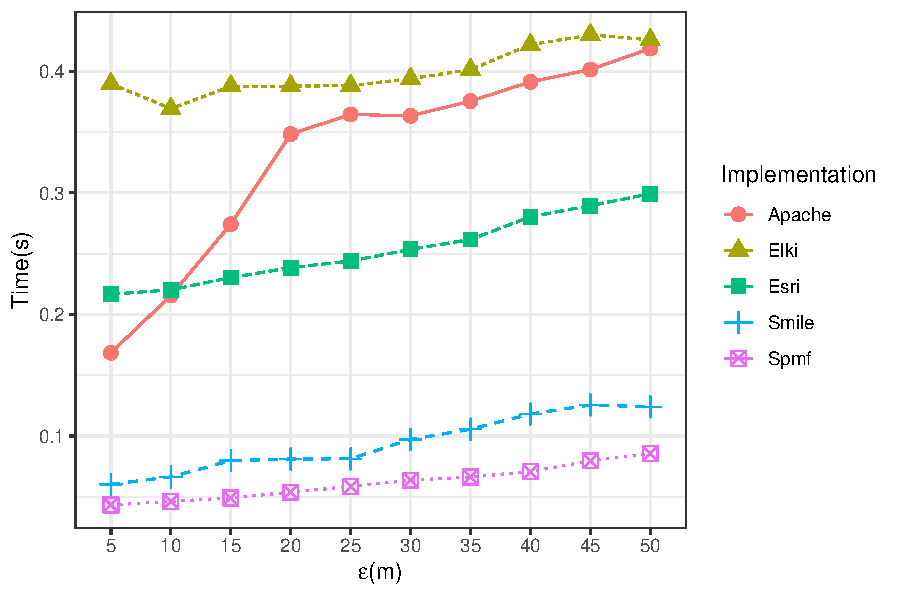
\includegraphics[width=0.6\textwidth]{figures/DBScanByTime}
\end{frame}

\begin{frame}{Dense areas}{Still problem in partition performance...}
    \centering
    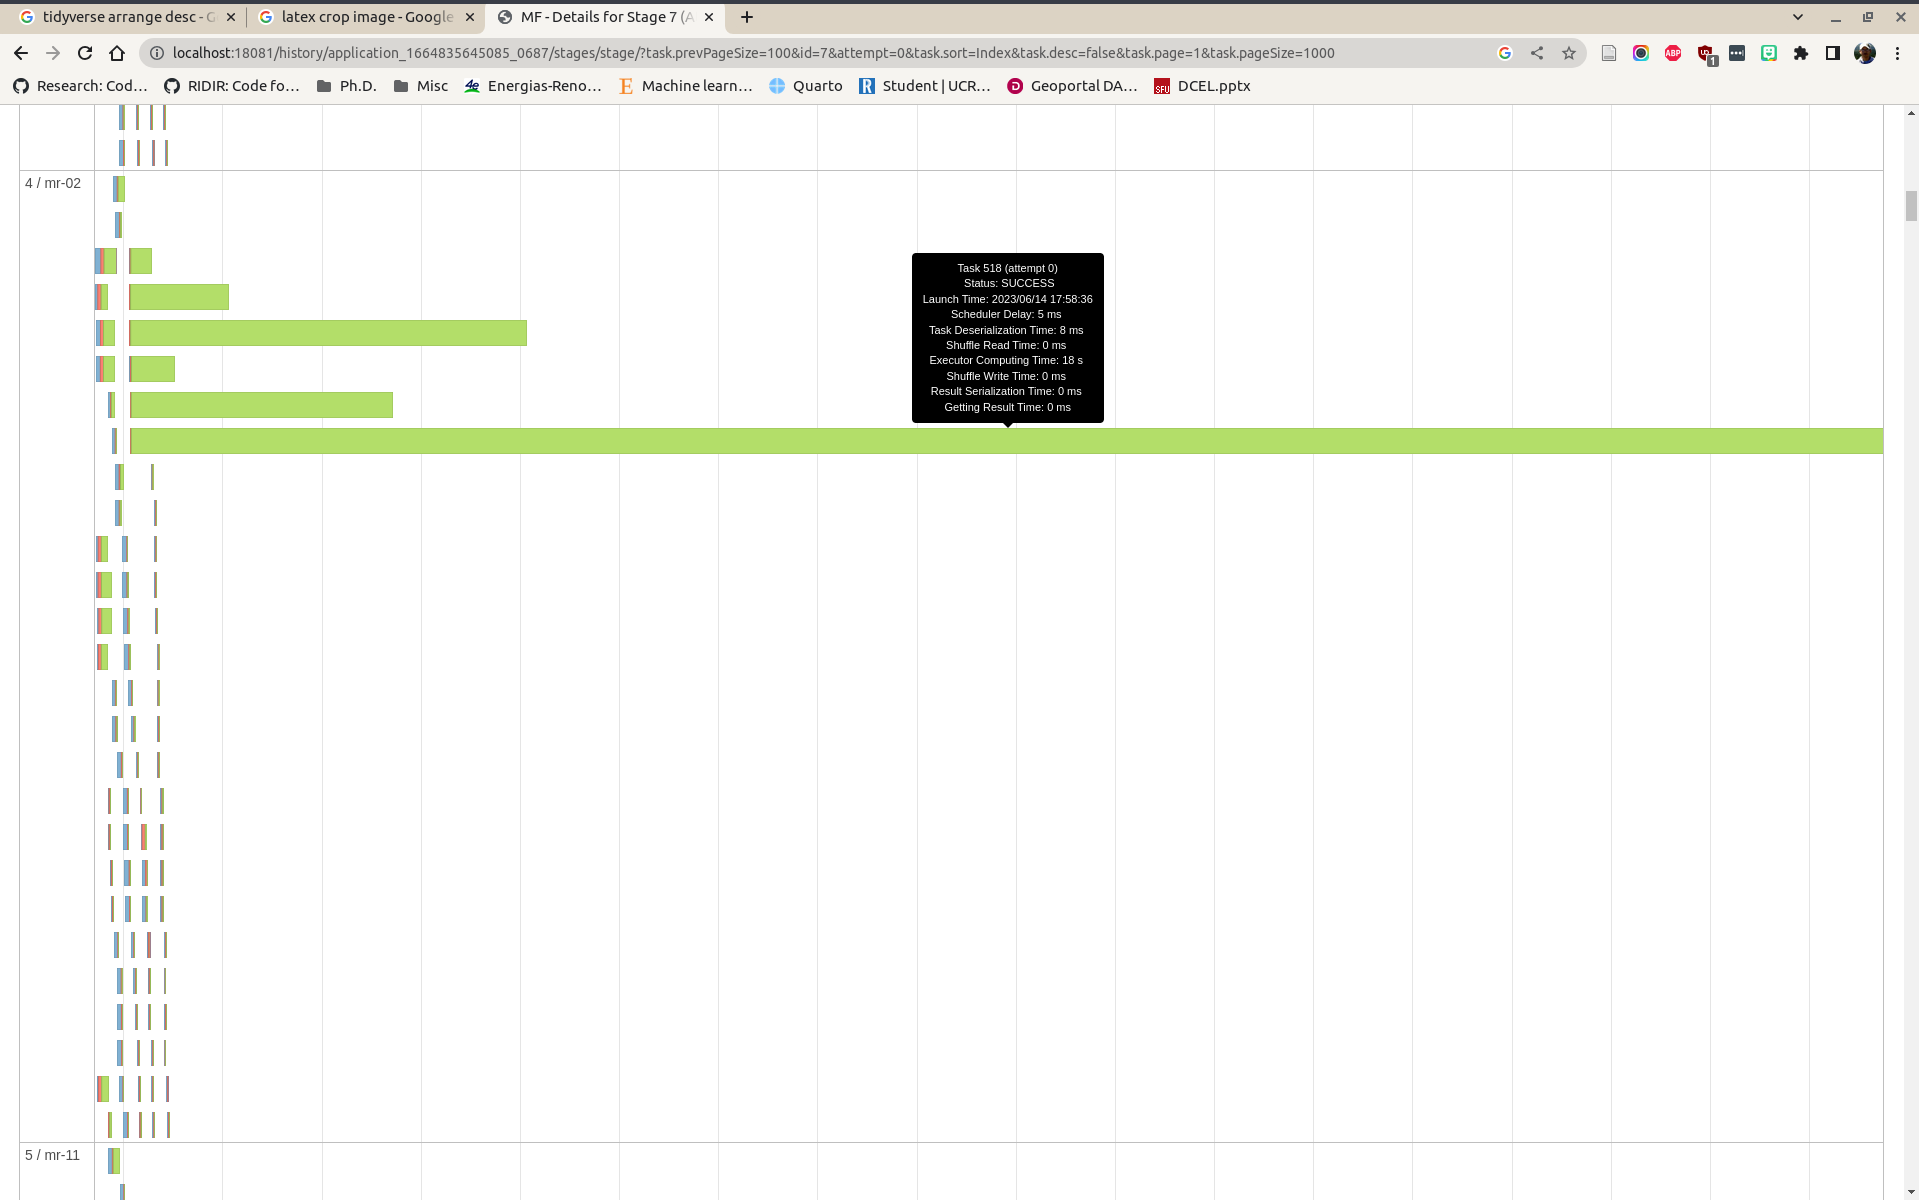
\includegraphics[width=0.9\textwidth]{figures/performance}
\end{frame}

\begin{frame}{Dense areas}{Having a look at problematic cells...}
    \centering
    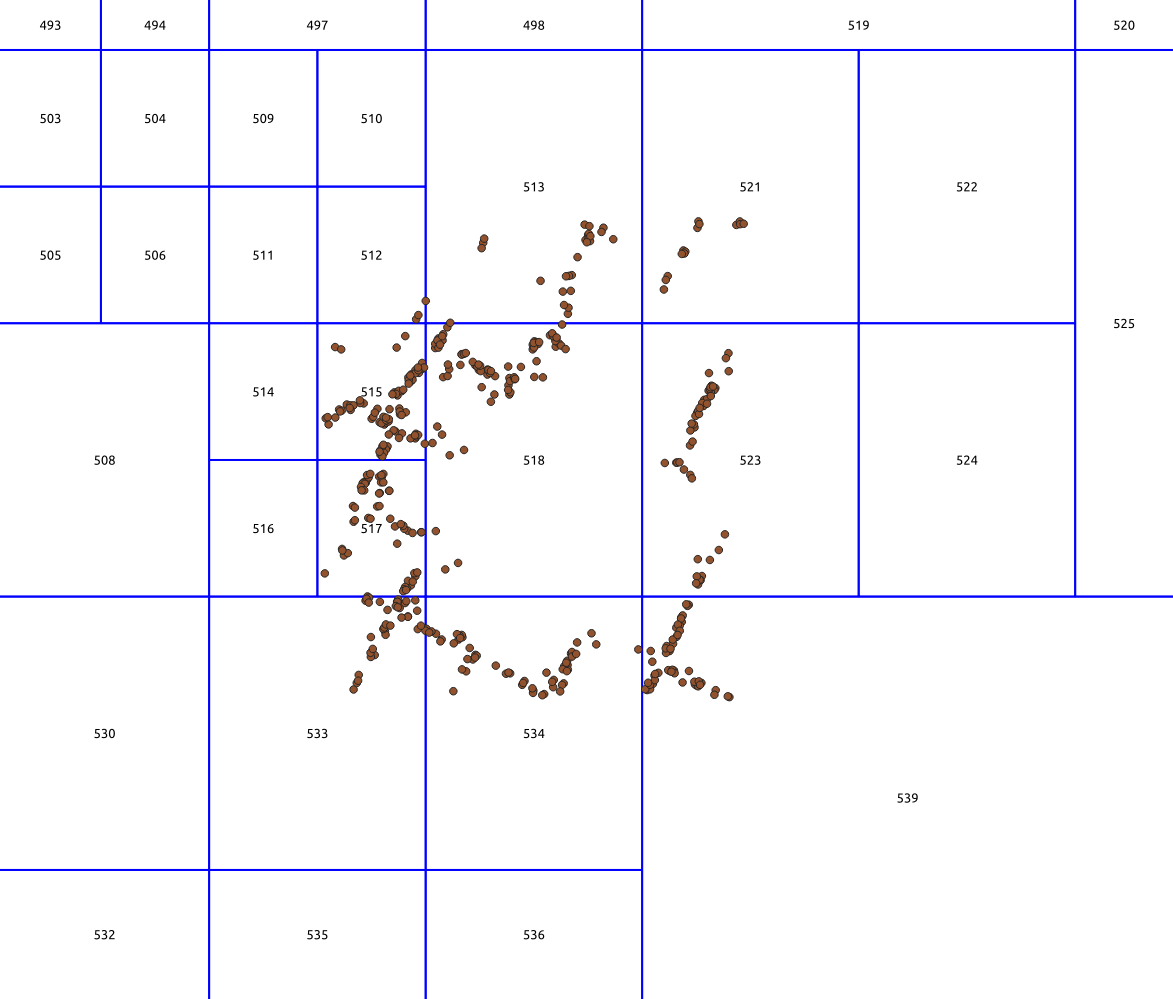
\includegraphics[width=0.7\textwidth]{figures/cell518}
\end{frame}

\begin{frame}{Dense areas}{Some stats for Cell 518...}
        \begin{table}[ht]
                \centering
                \begin{tabular}{ll}
                        \hline
                        \textbf{Stage} & \textbf{Number} \\
                        \hline
                        Points      & 455 \\
                        Pairs       & 11603 \\
                        Centers     & 23206 \\
                        Candidates  & 23049 \\
                        Maximals    & 558 \\
                          \hline
                \end{tabular}
        \end{table}
        \begin{table}[ht]
                \centering
                \begin{tabular}{ll}
                        \hline
                        \textbf{Stage} & \textbf{Time(s)} \\
                        \hline
                        Grid       & 0.0126 \\
                        Read       & 0.0050 \\
                        Pairs      & 0.0328 \\
                        Centers    & 0.3852 \\
                        Candidates & 0.0095 \\
                        Maximals   & 11.8734 \\
                        \textbf{Total}      & \textbf{12.4339} \\
                        \hline
                \end{tabular}
        \end{table}
\end{frame}

\begin{frame}{Dense areas}
    \centering
    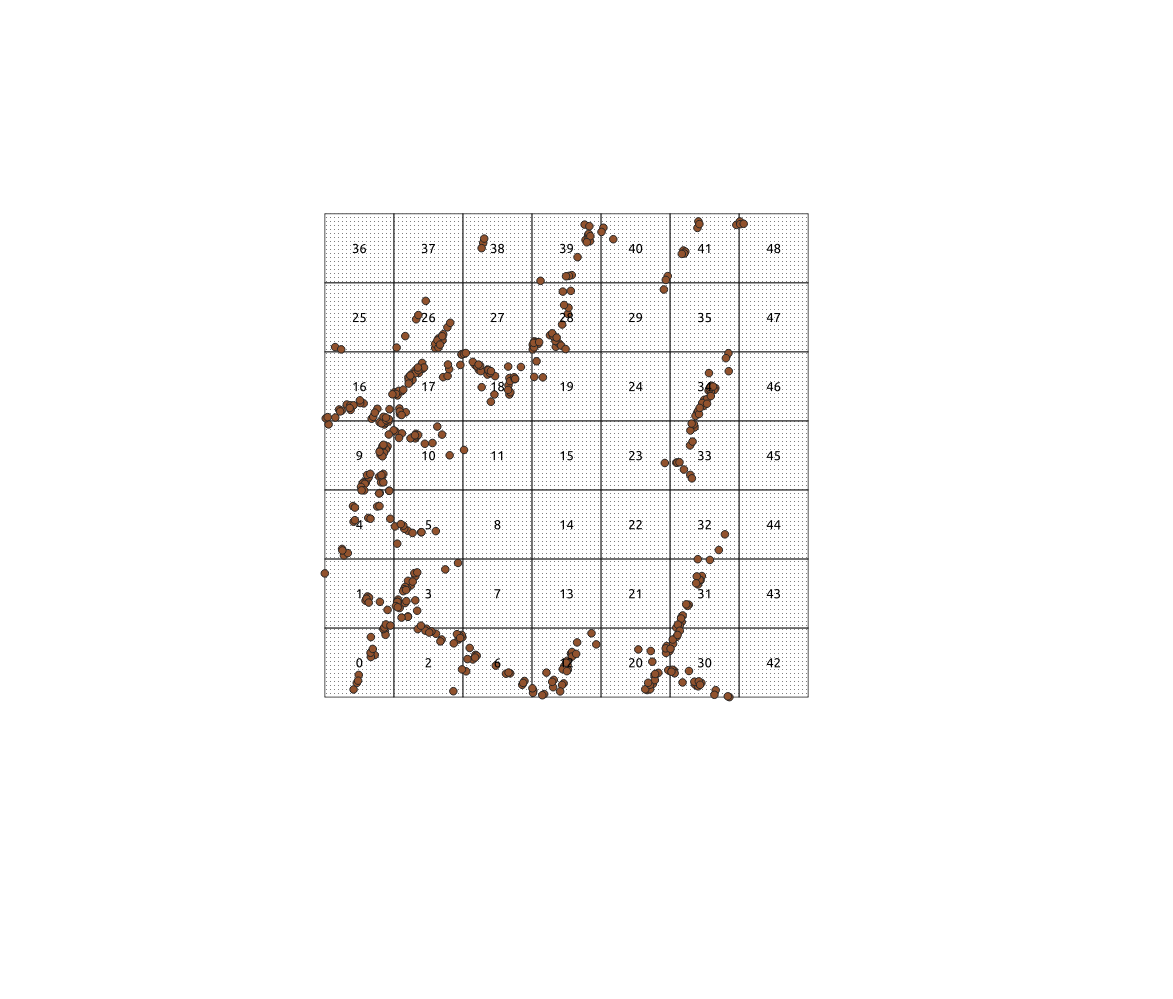
\includegraphics[trim={300 300 300 210}, clip, width=0.6\textwidth]{figures/cell518_grids}
\end{frame}

\begin{frame}{Dense areas}{Top 10 longest duration grids inside Cell 518...}
        \begin{table}[ht]
                \centering
                \begin{tabular}{r r c r r}
                        \hline
                        & \textbf{Id} & \textbf{Position} & \textbf{Points} & \textbf{Time(s)} \\
                        \hline
                        1 & 17 & (1,4) & 156 & 3.67 \\
                        2 & 9 & (0,3) & 135 & 3.05 \\
                        3 & 16 & (0,4) & 125 & 1.18 \\
                        4 & 18 & (2,4) & 124 & 0.99 \\
                        5 & 10 & (1,3) & 166 & 0.58 \\
                        6 & 3 & (1,1) & 111 & 0.48 \\
                        7 & 26 & (1,5) & 110 & 0.47 \\
                        8 & 20 & (4,0) & 88 & 0.26 \\
                        9 & 4 & (0,2) & 116 & 0.21 \\
                        10 & 0 & (0,0) & 68 & 0.17 \\
                        \hline
                \end{tabular}
        \end{table}
\end{frame}

\begin{frame}{Dense areas}{Longest duration grid...}
    \centering
    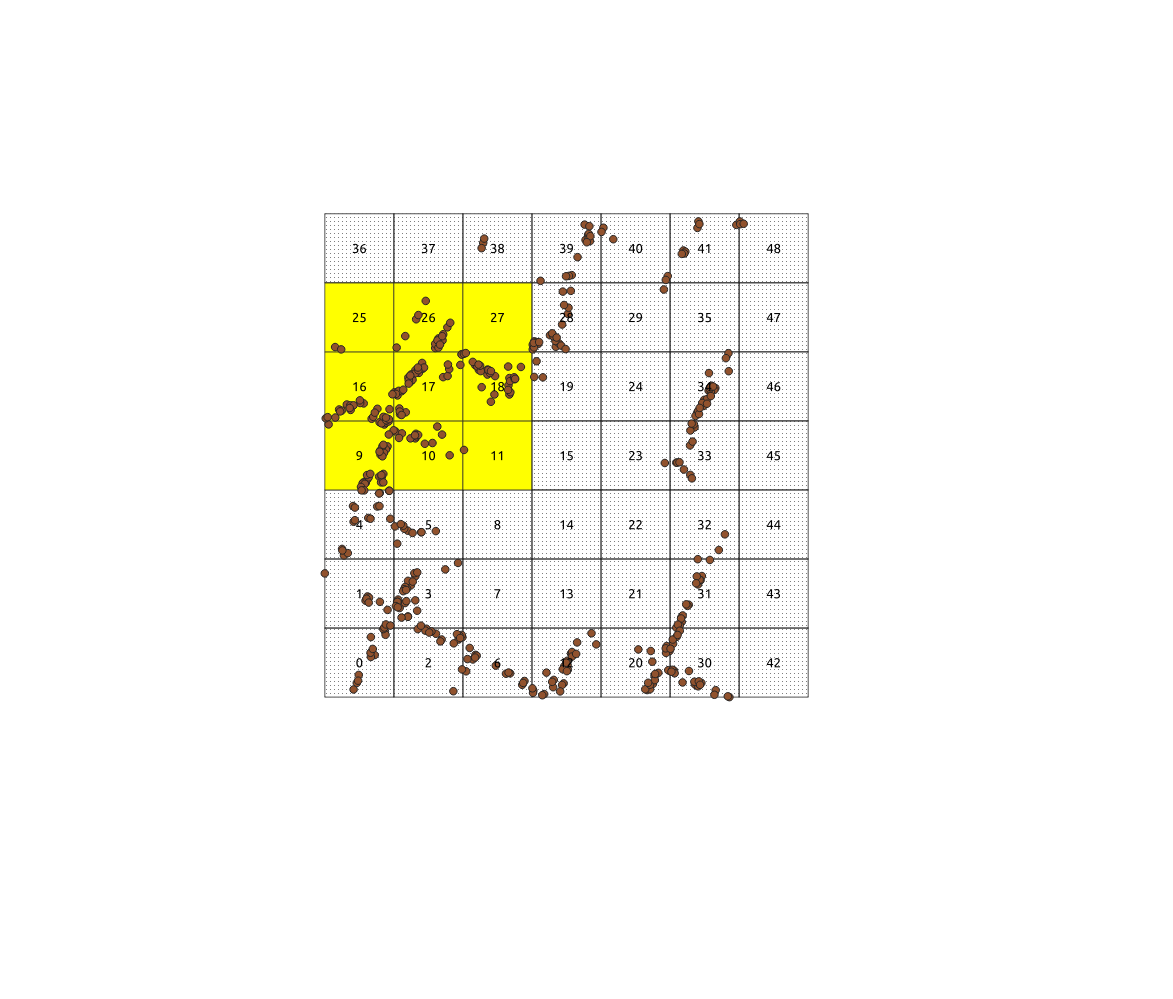
\includegraphics[trim={300 300 300 210}, clip, width=0.6\textwidth]{figures/cell518_grid17}
\end{frame}

\begin{frame}{Dense areas}{Number of points and duration per grid...}
        \centering
        \begin{minipage}{0.49\textwidth}
                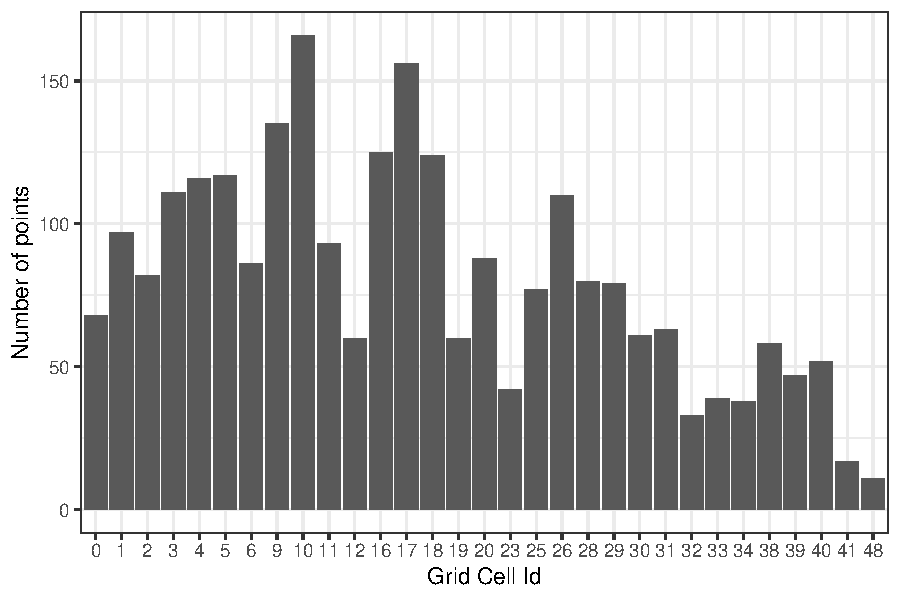
\includegraphics[width=\textwidth]{figures/hoods518_n}
        \end{minipage}
        \begin{minipage}{0.49\textwidth}
                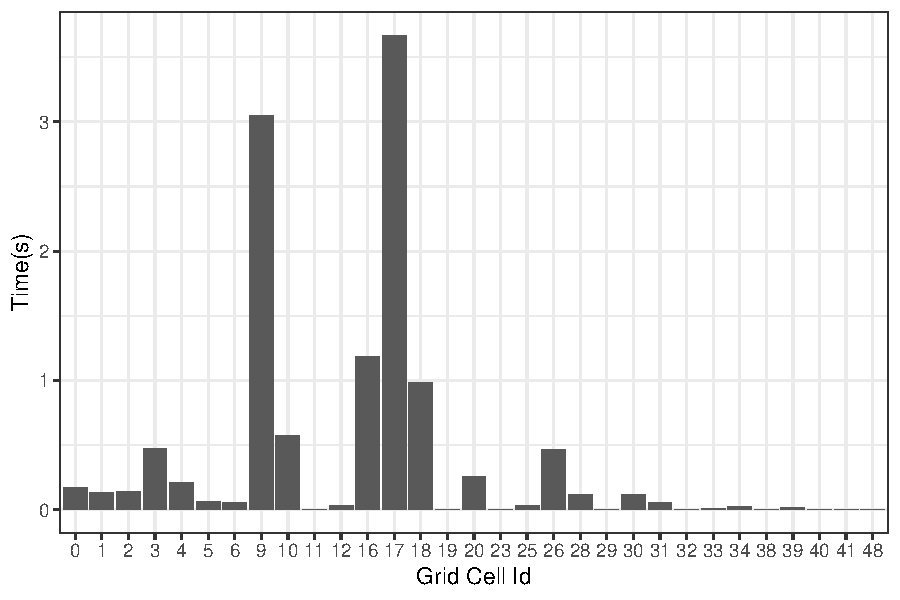
\includegraphics[width=\textwidth]{figures/hoods518_time}
        \end{minipage}
\end{frame}

\begin{frame}{Dense areas}{Duration per grid...}
    \centering
    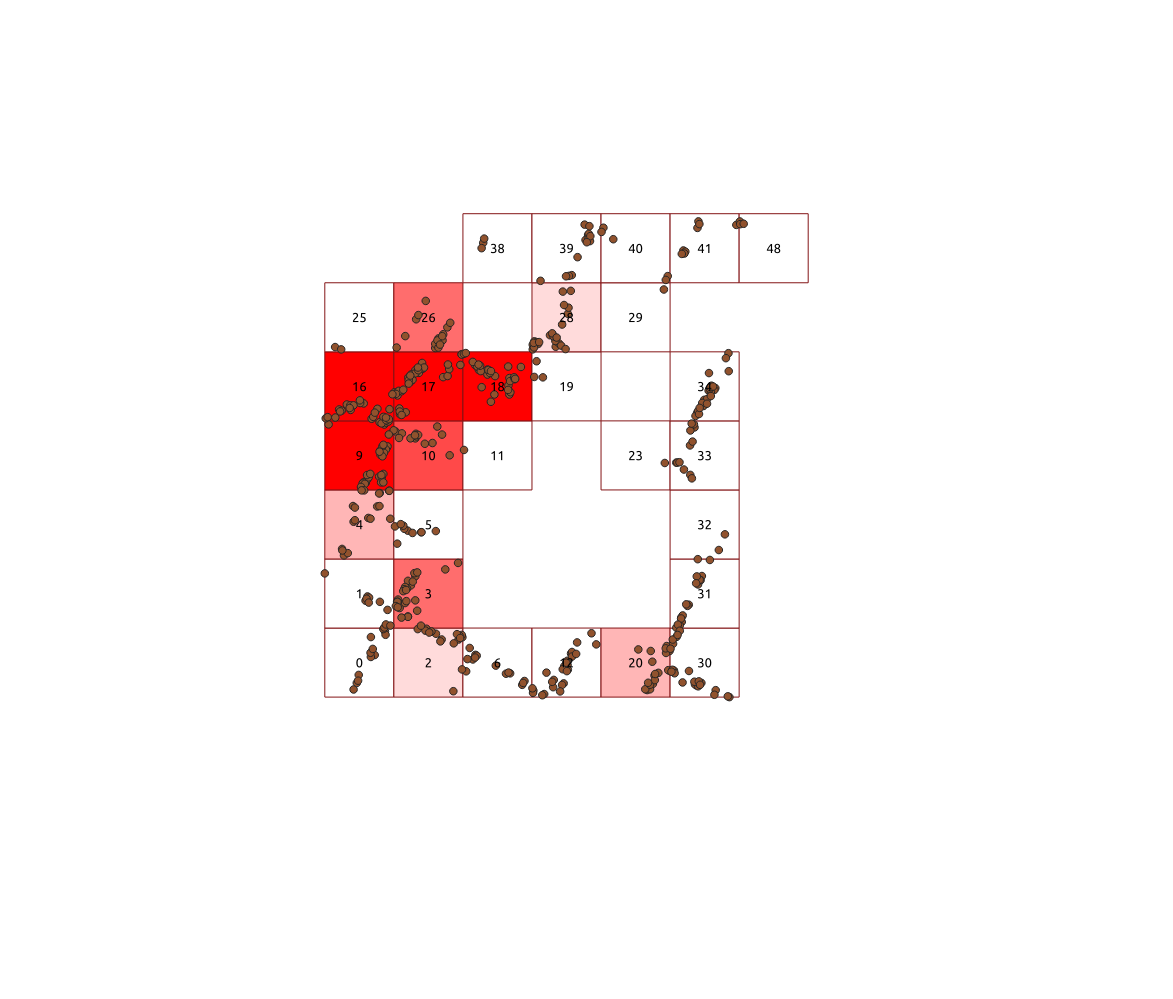
\includegraphics[trim={300 300 300 210}, clip, width=0.6\textwidth]{figures/cell518_grid_times}
\end{frame}

\begin{frame}{What is next...}
        \begin{itemize}
                \item Working on distributing the neighborhoods in dense areas...
                \item Defining a metric to consider an area as \textit{``dense''}...
                \item Validating and testing performance in cluster...
                \item Exploring strategies to improve cell replication for large $\varepsilon$ values...
        \end{itemize}
\end{frame}

\end{document}

